\documentclass[a4paper]{article}
%\usepackage[margin=2cm]{geometry}

\usepackage[catalan]{babel} % Language 
\usepackage{amsmath}
\usepackage{amssymb}
\usepackage{amsfonts}
\usepackage{fontspec}
\usepackage{graphicx}
\usepackage[makeroom]{cancel}
\usepackage{float}
\usepackage{enumerate}
\usepackage{mathtools}
\usepackage{tikz}
\usepackage{pgfplots}

\setlength{\parindent}{0pt}
\setlength{\parskip}{0.2cm}

\title{Tema 4: Models lineals per regressió}
\author{Joan Marcè Igual}

\begin{document}
\maketitle

\section{Introducció}
El problema de la regressió consisteix en, donat un vector $x \in \mathbb{R}^d$, predir un escalar $t \in \mathbb{R}$, on la relació (la dependència) entre $t$ i $x$ és estocàstica, així doncs escrivim:


\begin{align*}
t = f(x) + \varepsilon,\ \varepsilon &\text{ variable aleatòria} \\
i) \quad &\mathbb{E}(\varepsilon) = 0 \\
ii)\quad & Var(\varepsilon) = \sigma^2 < \infty
\end{align*}

Veiem unes dades:

$$
\mathcal{D} = \{ (x_1, t_1), ... (x_n, t_n)  \} \quad x_n \in R^d, t_n \in R^d \quad m.a.s.
$$

\textbf{Exemple:} ajust polinòmic

$$
y(\boldsymbol{x}, \boldsymbol{c}) = c_0 + \sum_{i=1}^M c_i x^i \quad x \in \mathbb{R}
$$
$$
x \in \mathbb{R}^d\ ? \text{ els polinomis \textbf{no escalen} a més d'una variable}
$$

Introduïm el concepte de \textbf{funcions de base}

$$
\phi_i: \mathbb{R}^d \rightarrow \mathbb{R}, \quad i = 1,...,M
$$
\begin{align*}
y(\textbf{x}, \boldsymbol{w}) &= w_0 + \sum_{i=1}^{M-1} w_i \phi_i (\textbf{x}) \\
&=  \sum_{i=0}^{M-1} w_i \phi_i (\boldsymbol{x}), \quad \phi_0 (\boldsymbol{x}) = 1
\end{align*}
\textbf{Exemple:} $\phi_i (x) = x^i$

Escrivim
$$
y(\boldsymbol{x}, \boldsymbol{w}) = \sum_{i=0}^{M-1} w_i \phi_i (\boldsymbol{x}) = \boldsymbol{w}^T \boldsymbol{\phi} (\boldsymbol{x})
$$

$$
\boldsymbol{w} = 
\begin{pmatrix}
w_0 \\ w_1 \\ \vdots \\ w_{M-1}
\end{pmatrix};\quad
\boldsymbol{\phi}(\boldsymbol{x}) = 
\begin{pmatrix}
\phi_0 (\boldsymbol{x}) = 1 \\
\phi_1 (\boldsymbol{x}) \\
\vdots \\
\phi_{M-1} (\boldsymbol{x})
\end{pmatrix}
$$

\section{Regressió clàssica}

$$
\varepsilon \sim N(0, \sigma^2)
$$

Si tenim una distribució normal (veure figura 1) l'amplada del pic de la gaussiana depèn de $\sigma^2$.

\begin{figure}[H]
    \centering
    \begin{tikzpicture}
        \begin{axis}[samples=200]
            \addplot+[mark=none] {1/(sqrt(2*pi)) * exp(-(x^2)/2)};
            \addplot+[mark=none] {1/(2*sqrt(2*pi)) * exp(-(x^2)/8)};
            \legend{$\sigma = 1$, $\sigma = 2$};
        \end{axis}
    \end{tikzpicture}
\end{figure}

$ t = f(x) + N(0, \sigma^2) $ és equivalent a escriure $T \sim N(f(x), \sigma^2) $.

Així doncs si s'agafa la mitjana de $x$ i s'uneixen els punts, la funció resultant és la millor possible. Així doncs la funció de regressió $f^*(x) = \mathbb{E}(T|X)$.

L'únic que ens falta és posar les dades en una matriu:

$$
X_{N \times d} =
\begin{pmatrix}
\longleftarrow x_1 \longrightarrow \\
\longleftarrow x_2 \longrightarrow \\
\vdots \\
\longleftarrow x_N \longrightarrow
\end{pmatrix}
$$

D'aquesta manera tenim $\mathcal{D}$ conegudes $(x_n, t_n)$, $w$ i $\sigma^2$ desconeguts, per tant apliquem \textbf{Màxima Versemblança}.

$$
\theta = (w, \sigma^2)
$$

\begin{gather*}
-\ell (\theta) = -ln \mathcal{L} (\theta) = 
-ln \mathcal{L}(w, \sigma^2) =
-ln P(t | X, w, \sigma^2) \underbrace{=}_{m.a.s.} \\
-ln \prod_{n=1}^N P(t_n | x_n, w, \sigma^2) \underbrace{=}_{modelat}
-ln \prod_{n=1}^N \mathcal{N} (t_n, y(x_n, w), \sigma^2) =
- \sum_{n=1}^N ln \ \mathcal{N} (t_n, y(x_n, w), \sigma^2) = \\
- \sum_{n=1}^N \left\{ ln \left( \frac{1}{\sqrt{2\pi}\sigma} \right) - \frac{(t_n - y(x_n, w))^2}{2\sigma^2} \right\} = 
\sum_{n=1}^N \left\{ ln(\sqrt{2\pi}\sigma) + \frac{(t_n - y(x_n, w))^2}{2\sigma^2} \right\} = \\
N ln (\sqrt{2\pi}) + \frac{1}{2\sigma^2} \sum_{n=1}^N (t_n - y(x_n,w))^2 \text{ és equivalent a } \frac{1}{2} \sum_{n=1}^N (t_n - y(x_n, w))^2 = E(w)
\end{gather*}

$$
\boxed{y(x, \boldsymbol{w}) = \boldsymbol{w}^T \Phi(x)} \text{ és convinent }
$$

$$
\Phi_{N \times M} =
\begin{pmatrix}
\phi_0 (x_1) & \phi_1(x_1) & \ldots & \phi_{M-1} (x_1) \\
\phi_0 (x_2) & \phi_1(x_2) & \ldots & \phi_{M-1} (x_2) \\
\vdots & \vdots & \ddots & \vdots \\
\phi_0 (x_N) & \phi_1(x_N) & \ldots & \phi_{M-1} (x_N)
\end{pmatrix}
\text{ matriu de disseny}
$$

$$
\mathcal{N}(t, \mu, \sigma^2) = \frac{1}{\sqrt{2 \pi} \sigma} exp \left( - \frac{(t - \mu)^2}{2\sigma^2} \right)
$$

Expressem \textbf{l'error quadràtic}
$$
E(w) = \frac{1}{2} || \boldsymbol{t} - \Phi \boldsymbol{w} ||^2 = \frac{1}{2} \left\{ ||\boldsymbol{t}||^2 + ||\Phi \boldsymbol{w}||^2 - 2t^T(\Phi \boldsymbol{w}) \right\}
$$

$$
\frac{\partial E}{\partial \boldsymbol{w}} = \frac{1}{2} \left\{ 0 + 2 \Phi^T \Phi \hat{\boldsymbol{w}} - 2 \Phi^T \boldsymbol{t} \right\} = \Phi^T \Phi \hat{\boldsymbol{w}} - \Phi^T \boldsymbol{t} = \boldsymbol{0} \implies
$$
$$
\left( \Phi^T \Phi \right) \hat{\boldsymbol{w}} = \Phi^T \boldsymbol{t} \implies
\boxed{\hat{\boldsymbol{w}} = (\Phi^T \Phi)^{-1} \Phi^T \boldsymbol{t}} =
\Phi^{\dag} \boldsymbol{t}
$$
$$
\frac{\partial E}{\partial \sigma^2} = \frac{1}{N} \sum_{n=1}^N (t_n - \boldsymbol{w}^T \phi(x_n))^2 = \frac{2}{N} E(w)
$$

\textbf{Teorema} ("mínims quadrats")
Sigui $\Phi_{N\times M}, \quad N > M$. Si els vectors columna de $\Phi$ són linealment independents, és a dir, $rang(\Phi) = M$ (\emph{full rank}), llavors:

\begin{enumerate}
	\item La matriu $\Phi^T\Phi$ és simètrica i semi-definida positiva
	\item El problema de mínims quadrats: 
	$\underset{\boldsymbol{w}}{min} ||\boldsymbol{t} - \Phi \boldsymbol{w}||^2$ té solució única.
	\item Per trobar-la, cal resoldre el sistema d'equacions: $\Phi^T\Phi \boldsymbol{w} = \Phi^T \boldsymbol{t}$ (equacions normals de'n Gauss)
\end{enumerate}

La matriu $ \Phi^{\dag} := \left( \Phi^T \Phi \right)^{-1} \Phi^T $ és pseudo-inversa (inversa de Moore-Penrose) $ \Phi^{\dag} \Phi = I $

\section{La Descomposició en Valors Singulars (SVD)}

La solució de la regressió lineal requereix el càlcul de la matriu pseudo-inversa de la matriu de disseny ($\Phi$):

$$ \Phi^{\dag} := ( \Phi^T \Phi)^{-1} \Phi^T \qquad \Phi_{N \times M \ (N > M)} $$

El càlcul directe té dos problemes:
\begin{enumerate}[i)]
	\item $\Phi^T \Phi$ és $M \times M$; la inversió d'aquesta matriu és un procés numèric subjecte a errors de precisió. Si $M$ és gran, el cost computacional es dispara $\rightarrow O(M^3)$.
	\item Tot i tenir inversa si la matriu $\Phi^T \Phi$ està a prop de ser singular (està a prop de no tenir inversa) el procés d'inversió és delicat numèricament.
\end{enumerate}

Així doncs prenem una matriu $\Phi_{N \times M, \ N > M}$. Qualsevol tal matriu es pot expressar com:

$$
\Phi = U \Delta V^T
$$

\begin{itemize}
	\item $U_{N \times M}$ i conté els \textbf{vectors propis} de la matriu $\Phi \Phi^T$, per columnes ($U$ és \textbf{ortogonal}: $U U^T = U^T U = I$)
	\item $V_{M \times M}$ i conté els \textbf{vectors propis} de la matriu $\Phi^T \Phi$, per columnes ($V$ és \textbf{ortogonal})
	\item $\Delta$ és una matriu quasi-diagonal:
	$$
	\begin{pmatrix}
	\lambda_1 & 0 & \cdots &  0 \\
	0 & \lambda_2 & \ddots &  \vdots \\
	\vdots & \ddots & \ddots & 0 & \\
	0 & \cdots & 0 &\lambda_r \\
	0 & \cdots & \cdots & 0 \\
	\vdots & & & \vdots \\
	0 & \cdots & \cdots & 0
	\end{pmatrix}
	$$
	
	\item  $r = rang(\Phi) \le min(N,M) = M$ $\lambda_i$ són les arrels quadrades dels valors propis de la matriu $\Phi^T \Phi$ (tots ells són $\ge 0$) $\implies \lambda_1, ...,\lambda_r > 0$.
\end{itemize}

\textbf{Teorema:} Donat un problema de mínims quadrats $ \Phi \boldsymbol{w} = \boldsymbol{t} $, on cal minimitzar $ ||\boldsymbol{t} - \Phi \boldsymbol{w} ||^2 $ respecte $\boldsymbol{w}$, la solució es pot trobar fent:

$$
\hat{\boldsymbol{w}} = V · diag \underbrace{\left( \frac{1}{\lambda_i}\right)_+}_{
	\mathclap{
		\begin{cases}
			\frac{1}{\lambda_i} &\text{ si } \lambda_i > 0 \\
			0 & \text{ si } \lambda_i = 0
		\end{cases}}} · U^T · \boldsymbol{t}
$$

\textbf{Demostració:}

\begin{align*}
\hat{\boldsymbol{w}} &= \left( \Phi^T \Phi \right)^{-1} \Phi^T \boldsymbol{t} =
\left[ \left( U \Delta V^T \right)^T \left( U\Delta V^T \right) \right]^{-1}
\left(U\Delta V^T\right)^T \boldsymbol{t} \\
& = \left[ V\Delta \cancel{\left( U^T U \right)} \Delta V^T \right] 
\left( V \Delta U^T \right) \boldsymbol{t} = 
\left( V \Delta^2 V^T \right)^{-1} \left( V \Delta U^T \right) \boldsymbol{t} \\ 
&=
\left( V \Delta^{\cancel{-2}} \cancel{V^T} \right) \left( \cancel{V} \cancel{\Delta} U^T \right) \boldsymbol{t} =
V \Delta^{-1} U^T \boldsymbol{t} = 
\boxed{V diag\left(\frac{1}{\lambda_i}\right)_+ U^T \boldsymbol{t}}
\end{align*}

\subsection{Regressió lineal regularitzada}

\textbf{Objectiu:} tenir un control explícit de l'ajust.

\begin{align*}
    & E_{\lambda} (\boldsymbol{w}) := E(\boldsymbol{w}) + \underbrace{\frac{\lambda}{2}}_{\mathclap{\text{ct. regularització}}}·||\boldsymbol{w}||^2, \ \lambda > 0 \\
    & E_{\lambda}(\boldsymbol{w}) = \frac{1}{2} || t - \Phi w ||^2 + \frac{\lambda}{2} || \boldsymbol{w} ||^2
\end{align*}
\begin{align*}
    & \frac{\partial E}{\partial \boldsymbol{w}} = 
    \Phi^T \Phi \boldsymbol{w} - \Phi^T \boldsymbol{t} \implies
    \frac{\partial E}{\partial \boldsymbol{w}} = 
    \Phi^T \Phi \boldsymbol{w} - \Phi^T \boldsymbol{t} + \lambda \boldsymbol{w} = 0 \implies \\
    & \implies \Phi^T \Phi \boldsymbol{w} + \lambda \boldsymbol{w} = \Phi^T \boldsymbol{t} \implies
    \left( \Phi^T \Phi + \lambda I \right) \boldsymbol{w} = \Phi^T \boldsymbol{t} \implies \\
    & \implies \text{ si } \left( \Phi^T \Phi + \lambda \boldsymbol{w} \right)^{-1} 
    \text{ existeix, llavors: } \hat{\boldsymbol{w}} = 
    \left( \Phi^T \Phi + \lambda I \right)^{-1} \Phi^T \boldsymbol{t}
\end{align*}


\textbf{Avantatges:}

\begin{enumerate}[i)]
	\item La regularització permet expressar models més complexes del necessari i penalitzar l'excés de complexitat.
	$$
	\begin{cases}
		\lambda \rightarrow 0 &\text{sobreajusta} \\
		\lambda \rightarrow \infty &\text{infra ajust}
	\end{cases}
	$$
	
	\item $\left( \Phi^T \Phi + \lambda I \right)^{-1}$ sempre existeix, $\forall \lambda > 0$.
\end{enumerate}

\subsubsection{\textsc{Cross-Validation}}

\begin{figure}[H]
    \centering
    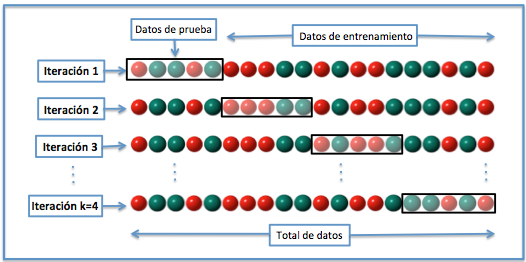
\includegraphics[width=0.8\textwidth]{images/K-fold_cross_validation}
    \caption{Representació de \textsc{Cross-Validation} amb $k=4$}
\end{figure}

Si es pinten totes les dades en un vector, cada punt és una fila de dades. S'escull un enter $K, \ 2 \le K \le N$. Si per exemple agafem $K=5$ dividim les dades en 5 parts. 

\verb|5-cross-validation| consistiria en fer 5 experiments. Les 4 primeres parts s'utilitzen per entrenar i la 5a part s'utilitza per validar les dades. Així es van fent experiments movent el conjunt de validació de lloc.

D'aquesta manera s'obtenen diferents errors de validació (5 errors diferents) que permeten obtenir l'error de validació creuada:
$$
error = \frac{1}{K} \sum_{i=1}^K va_i
$$

\textbf{Observacions:}
\begin{itemize}
	\item Totes les dades passen $K - 1$ vegades per entrenament i 1 vegada per validació.
	\item Els entrenaments que es fan no utilitzen totes les dades per entrenar degut a que s'utilitza un conjunt per validar.
	\item Si no hi ha \emph{cross-validation} només s'ha de fer un entrenament però utilitzant aquest mètode s'hauran de fer $K$ entrenaments.
\end{itemize}

Cas extrem: $\boldsymbol{K=N}$. A aquest mètode se li diu \textsc{Leave-One-Out-Cross-Validation} (LOOCV). En aquest mètode el biaix és petit i la variància és gran. Usat quan hi ha poques dades.

$\boldsymbol{K=2}$. Usant aquest valor de $K$ el biaix és gran i la variància és petita. Usat quan hi ha moltes dades.

$\boldsymbol{K=\{5,10\}}$. Aquest valor s'usa quan hi ha un valor mig de dades (ni moltes ni molt poques).

Tot i així és impossible trobar un valor òptim de $K$ ja que és molt difícil i realment no té molt sentit.

\verb|K-CV| s'utilitza per se\l.leccionar els millors hiper-paràmetres (paràmetres que el propi algoritme no pot optimitzar) d'una vàries tècniques $\rightarrow$ model selectiu.

Per exemple: proposar una seqüència de valors de $\lambda$ i provar-les totes calculant l'error de \verb|K-CV| per cadascuna.

Per \textbf{models lineals}, existeix una formula que calcula exactament l'error de LOOCV:
$$
error(LOOCV) = \frac{1}{N} \sum_{n=1}^N \frac{\left(t_n - y(x_n)\right)^2}{(1 - h_{nn})^2} \underset{\text{versió simplificada}}{\longrightarrow}
\frac{1}{N} \sum_{n=1}^N \frac{(t_n - y(x_n))^2}{\left(1 - \frac{Tr(H)}{N}\right)^2} = GCV
$$
$$
y(x_n) = \hat{\boldsymbol{w}}^T \boldsymbol{\phi} (x_n) \text{ (model lineal)}
$$
$$
H = (h_{ij}), \quad H = \Phi \Phi^{\dag} \text{ si no hi ha regularització}
$$
$$
H = \Phi \left( \Phi^T \Phi + \lambda I \right)^{-1} \Phi^T \text{ si hi ha regularització}
$$

\begin{itemize}
	\item Regressió regularitzada amb $||·||_2$:
	\begin{itemize}
		\item \textbf{matemàtic}: regularització de Tikhonov
		\item \textbf{APA}: regularització $L_2$
		\item \textbf{estadístic}: ridge regression
	\end{itemize}
	\item $||w||_1 = \sum_{i=1}^n |w_i|$
	
\end{itemize}
\end{document}